%--------------------------------------------------------------------
%
% Kanit Wongsuphasawat, Dominik Moritz
%
% Copied from Jeffrey Heer, Maneesh Agrawala, Nicholas Kong
% 
% Copied from James O'Brien's MICRO 2005 Continuation Proposal
%
%--------------------------------------------------------------------

\ProvidesFile{gp09.tex}
\documentclass[10pt,onecolumn,letterpaper]{article}
%\documentclass[11pt]{article}

\usepackage{times}
%\usepackage{palatino}
%\usepackage{arial}
\usepackage{graphicx}
\usepackage[font=small,justification=centering]{caption}
\usepackage{wrapfig}
\usepackage{fancyhdr}
\usepackage{cite}
\usepackage{ifthen}
\usepackage[usenames]{color}
\usepackage{url}

%--------------------------------------------------------------------

%\flushbottom

\setlength{\parindent     }{   0in}
\setlength{\parskip       }{.075in}

\setlength{\oddsidemargin }{-.1in}
\setlength{\evensidemargin}{-.1in}
\setlength{\topmargin     }{ -.1in}
%\setlength{\headsep       }{  .15in}
\setlength{\headsep       }{  .2in}
\setlength{\textheight    }{ 8.7in}
\setlength{\textwidth     }{ 6.5in}
\setlength{\parindent     }{   0in}
\setlength{\headheight    }{   0in}
\setlength{\parindent     }{   0in}

%--------------------------------------------------------------------
% Creating the pcode command for writing psuedocode
\newcommand{\pcline }{\rule{0in}{0.0in}    }  % Spacing for pseudo-code.
\newcommand{\pctab  }{\hspace{0.10in}      }  % Pseudo-code indentation.
\newcommand{\pcbigtab  }{\hspace{0.1in}    }  % Pseudo-code indentation.
\newcommand{\pcasgn }{\mbox{$\leftarrow$}  }  % Pseudo-code assignment operato
\newcommand{\pcomment}[1]{{\it #1}}  % Pseudo-code comments.

\newcommand{\pcode}[1]{
    \vspace{-0.1in}
    \begin{minipage}{100in} % The width argument will be ignored:
                            % See lamport p. 99
    \begin{tabbing} \hspace{0.20in} \= \pcbigtab \= \pcbigtab \= \pcbigtab \=
\pcbigtab \= \pcbigtab \= \\
       #1
    \end{tabbing}
    \end{minipage}
%    \vspace{0.15in}
}
%--------------------------------------------------------------------

\newcommand{\assA}{-1ex}
\newcommand{\assB}{-2ex}

\newcommand{\assAs}{-1ex}
\newcommand{\assBs}{-2ex}

\newcommand{\assAss}{-1ex}
\newcommand{\assBss}{-2ex}

\newcommand{\assAp}{-1ex}
\newcommand{\assBp}{-2ex}

\newcommand{\assAsp}{-1ex}
\newcommand{\assBsp}{-2ex}

\let\ORIGsection\section
\newcommand{\sectionname}{Section Name}
\def\section#1{\ifthenelse{\equal{#1}{*}}%
	{\sectionS}%
	{\renewcommand{\sectionname}{#1}\vspace{\assA}\ORIGsection{#1}\vspace{\assB}}}%
\def\sectionS#1{\renewcommand{\sectionname}{#1}\vspace{\assA}\ORIGsection*{#1}\vspace{\assB}}%

\let\ORIGsubsection\subsection
\def\subsection#1{\ifthenelse{\equal{#1}{*}}%
	{\subsectionS}%
	{\vspace{\assAs}\ORIGsubsection{#1}\vspace{\assBs}}}%
\def\subsectionS#1{\vspace{\assAs}\ORIGsubsection*{#1}\vspace{\assBs}}%


\let\ORIGsubsubsection\subsubsection
\def\subsubsection#1{\ifthenelse{\equal{#1}{*}}%
	{\subsubsectionS}%
	{\vspace{\assAss}\ORIGsubsubsection{#1}\vspace{\assBss}}}%
\def\subsubsectionS#1{\vspace{\assAss}\ORIGsubsubsection*{#1}\vspace{\assBss}}%


\let\ORIGparagraph\paragraph
\def\paragraph#1{\ifthenelse{\equal{#1}{*}}%
	{\paragraphS}%
	{\vspace{\assAp}\ORIGparagraph{#1}}}%
\def\paragraphS#1{\vspace{\assAp}\ORIGparagraph*{#1}}%


\let\ORIGsubparagraph\subparagraph
\def\subparagraph#1{\ifthenelse{\equal{#1}{*}}%
	{\subparagraphS}%
	{\vspace{\assAsp}\ORIGsubparagraph{#1}}}%
\def\subparagraphS#1{\vspace{\assAsp}\ORIGsubparagraph*{#1}}%

%--------------------------------------------------------------------
%--------------------------------------------------------------------

\newcommand{\Cite}[1]{\,\cite{#1}}

% Make the captions have small ``Figure #'' 
\makeatletter
\renewcommand{\@makecaption}[2]{%
        \vskip\abovecaptionskip
        {\small #1:} {\small #2\par
        \vskip\belowcaptionskip}}
\makeatother

\newcommand{\figureTop}[1]{
  \begin{figure}[!t]{\sloppy #1}\end{figure}
}

\newcommand{\figureBot}[1]{
  \begin{figure}[!b]{\sloppy #1}\end{figure}
}

\newcommand{\BM}[1]{
  \mbox{\boldmath$#1$}
}

\newcommand{\B}[1]{
  \mbox{\boldmath$#1$}
}

\newcommand{\TP}{^\mathsf{T}}
\newcommand{\IV}{^{-1}}
\newcommand{\TI}{^\mathsf{-T}}

\newcommand{\Unit}[1]{
 \mbox{$\,\mathrm{#1}$}
}

\newcommand{\Per}{\%} 
\newcommand{\Sec}{\,s} 
\newcommand{\Hz}{\,Hz} 


\newcommand{\Stress}{\ensuremath{\sigma}}
\newcommand{\StressD}{\ensuremath{{\Stress'}}}

\newcommand{\VMFC}{\ensuremath{\gamma_1}}
\newcommand{\VMFS}{\ensuremath{\gamma_2}}

\newcommand{\Strain}{\ensuremath{\epsilon}}
\newcommand{\StrainE}{\ensuremath{\epsilon^{(e)}}} 
\newcommand{\StrainP}{\ensuremath{\epsilon^{(p)}}}
\newcommand{\StrainRate}{\ensuremath{\dot{\Strain}}}
% Comment region command from Sara McMains
\newcommand{\comment}[1]{} 
% Make text red command (requires \usepackage[usenames]{color})
\newcommand{\textred}[1]{\textcolor{red}{#1}}
\newcommand {\note}[1]{{\color{magenta}\bf{Note: #1}\normalfont}}
% Turn comments into comments :)
\newcommand {\kanitw}[1]{{\color{red}\bf{KW: #1}\normalfont}}
\newcommand {\jheer}[1]{{\color{magenta}\bf{JH: #1}\normalfont}}
\newcommand {\dmoritz}[1]{{\color{blue}\bf{DM: #1}\normalfont}}



%--------------------------------------------------------------------

\begin{document}

\newlength{\origbaselineskip}
\setlength{\origbaselineskip}{\baselineskip}
%\setlength{\baselineskip}{.8\origbaselineskip}

%--------------------------------------------------------------------

\newcommand{\mytitle}{Accelerating Data Analysis with Visualization Recommendation}
\pagestyle{plain}  %Plain style with page numbes
%\pagestyle{empty}  %Plain style with no page numbers
%\pagestyle{fancy}
\lhead{\small\textsl{\mytitle}}
\rhead{}
\chead{}
\lfoot{}
\rfoot{}
%\cfoot{\small\textsl{Page \thepage}} % Add in page numbers
\cfoot{\small\textsl{}} % Remove page numbers
\renewcommand{\footrulewidth}{0pt}

\renewcommand{\thepage}{\arabic{page}}
\renewcommand{\thesection}{\Alph{section}}
%\renewcommand{\thesubsection}{\arabic{subSection}}

\fancypagestyle{plain}{
  \fancyhf{}
  \cfoot{\small\textsl{Page \thepage}} 
  \renewcommand{\footrulewidth}{0pt}
  \renewcommand{\headrulewidth}{0pt}
}


%--------------------------------------------------------------------
%--------------------------------------------------------------------


%--------------------------------------------------------------------
%--------------------------------------------------------------------
\clearpage

%--------------------------------------------------------------------
%--------------------------------------------------------------------

\clearpage


\newcommand{\abA}{4.25in}
\newcommand{\abO}{2.00in}
\newcommand{\abT}{2.75in}

\vspace{.10in}
\centerline{\Large \bf Accelerating Data Analysis with Visualization Recommendation}
% \vspace{.05in}
% \centerline{\Large \bf Validating Design Guidelines for Data Visualization}
\vspace{.10in}
\centerline{Kanit Wongsuphasawat and Dominik Moritz}
\vspace{-.1in}
\begin{center}
	{\bf Areas of Interests:} User Interfaces, Visualization, Recommender Systems, Data Analysis
\end{center}

% kanitw: do we need a citation here?
As business and academia become increasingly data-driven,
more and more data “analysts” may be novices in statistics and data visualization.
Accordingly, it becomes important for tools to better guide users towards
productive analytic processes and effectively designed visualizations.

For example, consider an analyst examining Broadband Internet Subscription per Population (\textit{Subscription}) over time in South American countries. As a line chart is a well-suited representation for temporal data, our system will recommend a line chart showing average \textit{Subscription} over \textit{Time} and another line chart showing \textit{Subscription} over \textit{Time} across different \textit{Countries}.  If the analyst becomes interested in the \textit{Subscription} in 2013, our system will subsequently present 2013 data as a sorted bar chart (to facilitate comparison) and also suggest a map (for investigating spatial relationships).  In addition, as \textit{Subscription} is correlated with each country’s \textit{GDP per capita}, our system will recommend a scatterplot to show the relationship between \textit{Subscription} and \textit{GDP per capita}.  With these suggestions (Figure 1), the analyst can quickly examine relationships and generate more hypotheses without having to manually instruct software to plot each chart one-by-one.


\begin{figure}[!htbp]
\centering
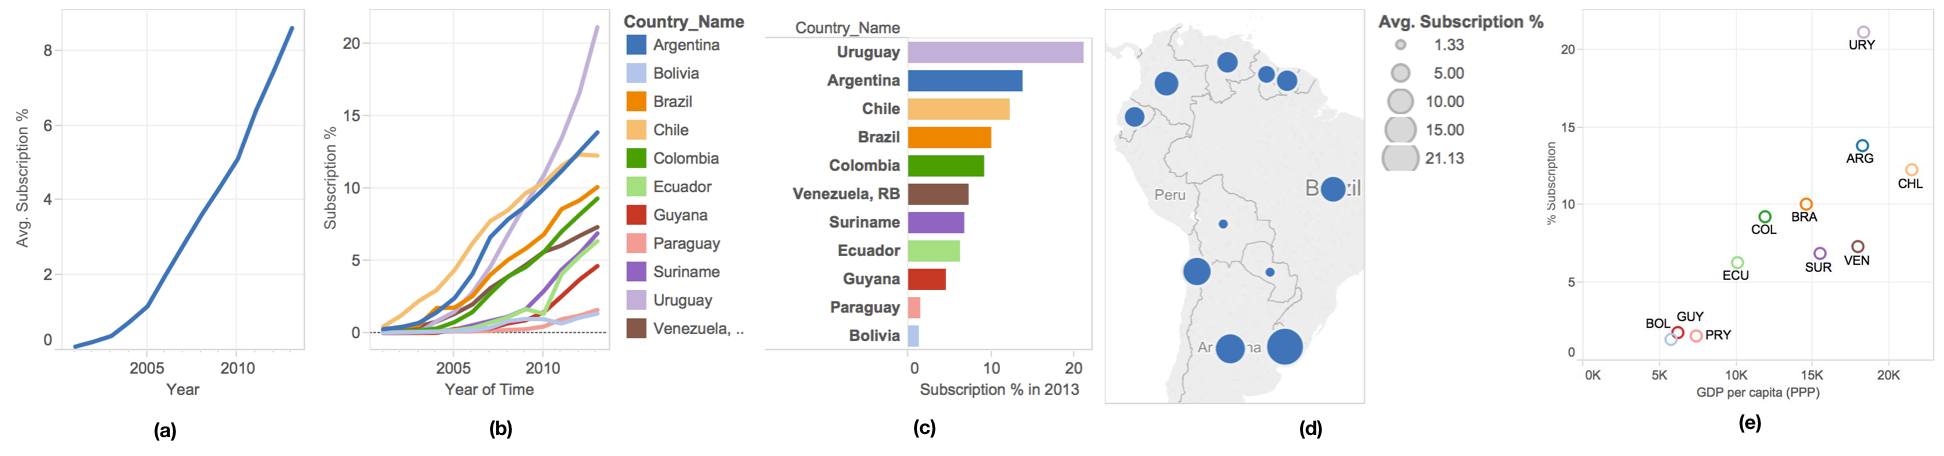
\includegraphics[width=6in]{figure1.png}
\vspace{-0.1in}
\caption{(a,b) line charts showing Broadband Internet Subscription per Population over time in South American countries (on average, and grouped by country respectively) (c,d) a bar chart and a map showing the Subscription in 2013 (e) a scatterplot showing relationship between Subscription and GDP per capita}
\label{fig-examples}
\vspace{-0.15in}
\end{figure}
\vspace{0.1in}

To augment analysts’ ability to perform data analysis, we propose to build a recommender system for visualizing relational data. The system will consist of the following components.

\textbf{1. Interface for Rapid Exploration.}
The interface will include expressive user controls for searching visualizations, enabling analysts to focus on iterative exploration and refinement rather than lower-level design details.

\textbf{2. Comprehensive Recommendation Algorithm.}  What makes a recommendation “good” depends both on the data and task at hand. Accordingly, we will develop a recommendation algorithm that balances user input, best practices (e.g., perceptual effectiveness rankings) for visualization design, data properties and diversity.

\textbf{3. Scalable System.} With larger data, current visualization systems become less responsive or even fail to run at all, preventing rapid exploration.  Furthermore, our recommender system will require expensive querying and modeling operations. We will develop a scalable client-server architecture with the goal of supporting interactive response rates.


\section*{Background}

It is often argued that the most effective visual analytics tools should support analysis at the rate of thought \cite{hanrahan:enthusiast}.
However, existing tools \cite{heer:dynamics} have not yet achieved this vision. \textit{Chart Typology} interfaces, such as a palette of chart templates found in spreadsheet software, are easy for view creation but difficult for view refinement.  \textit{Visualization Toolkits} \cite{bostock:d3, wilkinson:GoG} enable intricate designs but require coding, and therefore hinder rapid data exploration. Tableau \cite{stolte:polaris}, a state of the art visual analysis tool, enables rapid view exploration refinement and supports expressive visualizations creation.  However, creating an effective visualization in Tableau still requires both tool and design expertise.  To lower this barrier, Tableau's Show Me \cite{mackinlay:showme} feature automatically suggests suitable chart types for selected data attributes based on design practices \cite{tufte:visual, few:nowyouseeit}.  Nonetheless, it can suggest only a single visualization at a time although there are usually many appropriate visualizations.

A few research prototypes \cite{key:vizdeck, gotz:harvest, kandel:profiler} recommend a list of visualizations based on statistical properties of the data. While these systems may recommend relevant subsets of data, they produce only a limited range of visualizations and do not incorporate best practices of design.  Moreover, they lack interfaces for users to express their intention, leading to irrelevant suggestions.  An effective visualization recommender must address these limitations to successfully support users’ analysis.
\section*{User Interface}

\begingroup
\setlength{\columnsep}{16pt}

\begin{wrapfigure}{r}{4in}
\vspace{-0.3in}
\begin{center}
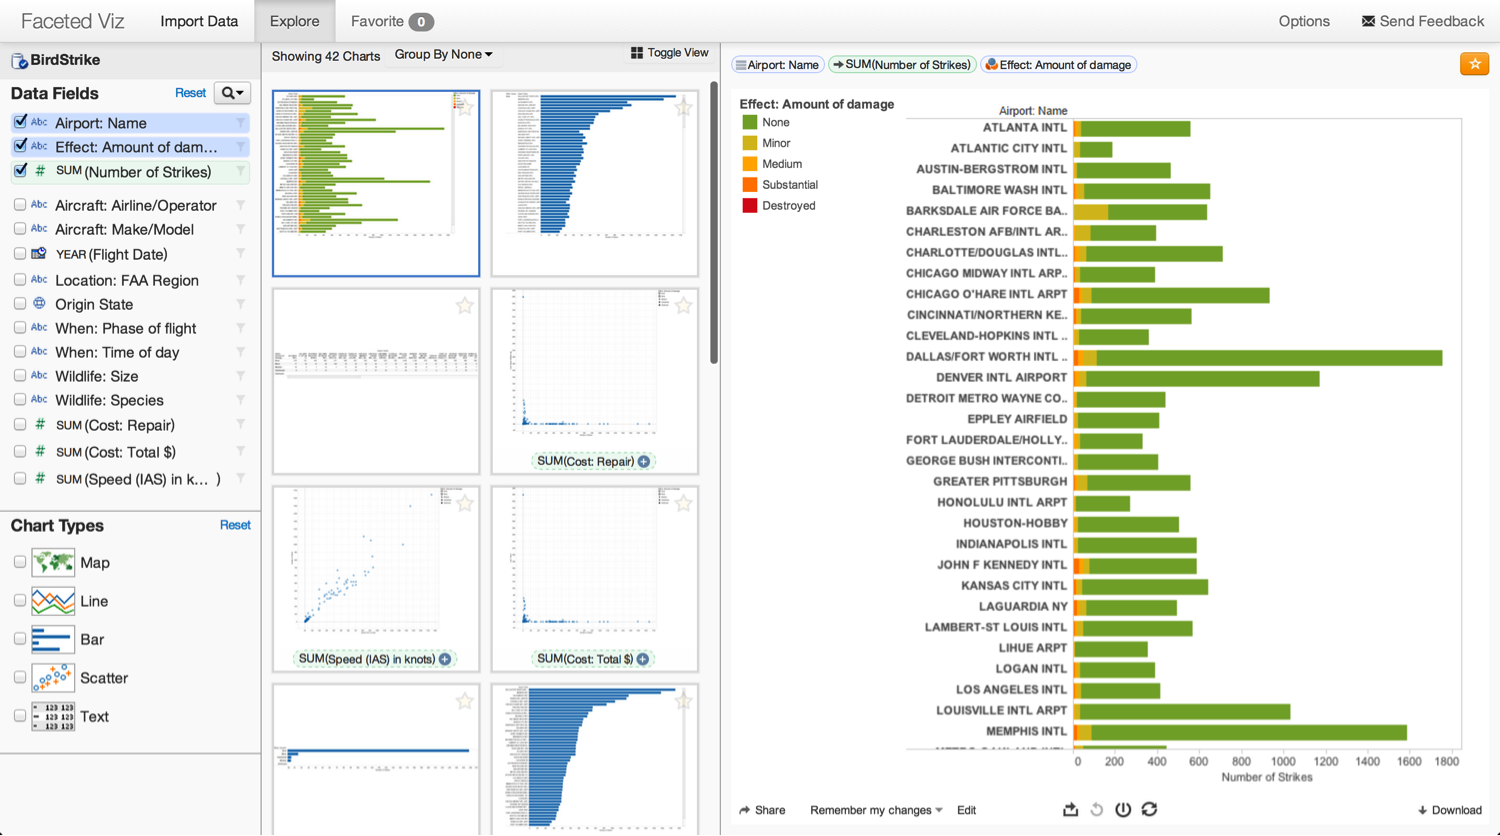
\includegraphics[width=4in]{ui.png}

\caption{Mock-up of our interface. Users can specify their query using controls on the left side.  The browser in the middle displays recommended visualizations.  The interactive view on the right shows the selected visualization.}
\label{fig:ui}
\end{center}
\vspace{-0.3in}
\end{wrapfigure}

Our system will help users focus on data exploration rather than design details by letting users search for visualizations.
Figure \ref{fig:ui} shows a mock-up of our interface. The interface will highlight data attributes and chart types as two main search facets \cite{yee:faceted}. Prior work indicates that people usually begin describing visualizations by specifying these two properties \cite{grammel:novice}.  Users can also specify data transformations and mappings between data attributes and visual variables. The browser view (Fig. \ref{fig:ui}, middle) will show recommended visualizations based on user input.  Users can then select and interact with a visualization of interest on the right side. The interface will also support the iterative nature of visual analysis.  Analysts can keep refining their queries with more specific intents.  Our interface will also provide annotation and provenance tools to support the analysis flow.


\endgroup

We will build an open-source, scalable, interactive visualization module for rendering visualizations, taking specifications generated by the recommendation algorithm as inputs. The module will incorporate design practices such as determining the optimal aspect ratio for the chart type and the data \cite{talbot:arc}.  Output views will support user interactions \cite{heer:dynamics} for data exploration such as highlighting, brushing and linking, zooming, and filtering. The views will also allow the recommender to automatically highlight inferred anomalies and trends.
\section*{Recommendation Algorithm}

The recommendation process will involve \textit{generation}, \textit{ranking} and \textit{pruning}.  The generation algorithm will create \textit{relevant} visualization specifications,  which includes permutations of possible mappings between data attributes and visual variables, and combinations of marks types and data transformations that match user queries.  The system will then rank visualizations using a quality metric that we will develop and evaluate as part of this research. Finally, as top-ranked visualizations may contain redundant information,  we will use a similarity metric to prune the results to ensure diversity.

Our quality metric will combine multiple criteria including \textit{design quality} and \textit{interestingness}. The \textit{design quality} score will integrate design guidelines based on graphical perception studies \cite{cleveland:perception}.  For example, in perceptual effectiveness rankings of visual encodings of quantitative data \cite{mackinlay:apt}, length is more effective than angle.  Therefore, our algorithm will a priori prefer bar charts to pie charts.  To determine an \textit{interestingness} score, we will apply statistical measures such as mutual information\cite{wang:maximum} as well as anomaly and trend detection\cite{chandola:anomaly}. We will explore the use of interpretable machine learning techniques \cite{letham:interpretable} to combine our metrics, enabling our system to explain why a particular view is recommended. In the long term, we will extend the algorithm to learn from user interactions.
\section*{Scalable System Architecture}

Our visualization system will use a client-server infrastructure with a web-based client. The backend server will use database techniques to efficiently store and query data for the visualizations. Data can reside in the client, the server's memory or in persistent storage.  We will develop a query optimizer that automatically determines whether a particular computation should be computed on the client or on the server based on data size, data location and latency.  A part of server resources will be allocated for profiling and finding explanations for anomalies and trends.  Finally, we will explore big data techniques including index precomputation and data cubes to support fast brushing and linking \cite{liu:immens, lins:nanocubes}, data reduction methods such as sampling to simplify complex data, and online aggregation \cite{hellerstein:onlineagg, agarwal:blinkdb, fisher:trustme} to enhance responsiveness for larger data. We believe that coupling database systems and interactive visualizations will be performant and enable new functionalities \cite{wu:dvms}.
\section*{One Year Horizon}

\begingroup
\setlength{\columnsep}{16pt}

\begin{wrapfigure}{r}{3in}
\vspace{-0.4in}

  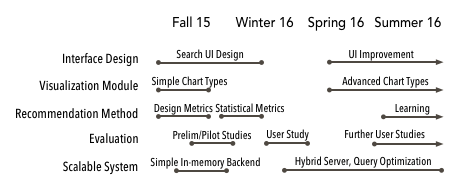
\includegraphics[width=3in]{gantt-chart.png}
  \vspace{-0.3in}
  \caption{Timeline during the 2015-2016 Academic Year}

\label{fig:plan}
\vspace{-0.1in}
\end{wrapfigure}


This research is a multi-year project.  We expect to deliver a working system for general datasets that fit in memory in the first year.

Figure 3 shows our project timeline during the 2015-2016 Academic Year.
We will initially focus on developing and evaluating user interfaces and recommendation algorithms.   The initial system will support commonly used chart types including histogram, bar chart, line chart, scatter plot and map.  We will perform a lab study comparing our recommender system with an existing tool such as Tableau.  We will measure the rate of events such as participants’ observations, generalizations and questions during the analysis sessions \cite{liu:latency}.

\endgroup

During the first half of the year, we will also start the implementation of the backend server.  In the latter half of the year, we will focus on scaling the system to support higher volume of data and advanced visualization types. We will also improve our user interface and recommender algorithm based on user study results, and run further user studies.



\section*{Team}

Our work will be a major step towards visualization systems that support analysis at the rate of thought.  For this kind of work to succeed, it is critical to have an interdisciplinary team with expertise in both Human-Computer Interaction and Data Management Systems. Our experience across these areas makes our team a strong candidate to tackle these challenges.  In addition, at the University of Washington we have strong collaborators in the Interactive Data Lab, the Database Group, and the eScience Institute.

\textbf{Kanit Wongsuphasawat} is a Ph.D. student in Computer Science \& Engineering and a member of the Interactive Data Lab at the University of Washington.  Kanit has expertise in Human-Computer Interaction and Visualization.  He is a co-developer of a declarative model for interactive visualization design \cite{satyanarayan:reactive-vega}.  Kanit has been awarded a Fulbright Fellowship and H.M. the King of Thailand scholarship.  He also has professional experience working in leading data-driven companies including Google, Tableau Software and Trifacta.

\textbf{Dominik Moritz} is a Ph.D. student in Computer Science \& Engineering at the University of Washington.   As a member of both the Database group and the Interactive Data Lab, Dominik has a strong background in data management systems and visualization.  He co-develops Myria, a distributed database system \cite{halperin:myria} and was a core developer of CKAN and creator of a number of libraries for data management and sharing. He has been awarded a Fulbright Fellowship and a scholarship from the German National Academic Foundation.

\bibliographystyle{acm-sigchi}
{\footnotesize
	\bibliography{qualcomm}
}
\end{document}

%--------------------------------------------------------------------
%--------------------------------------------------------------------

 



